\section{Intorduction to Docker}\label{intorduction-to-docker}

Docker is the company driving the container movement and the only
container platform provider to address every application across the
hybrid cloud. Today's businesses are under pressure to digitally
transform but are constrained by existing applications and
infrastructure while rationalizing an increasingly diverse portfolio of
clouds, datacenters and application architectures. Docker enables true
independence between applications and infrastructure and developers and
IT ops to unlock their potential and creates a model for better
collaboration and innovation.

\begin{figure}
\centering
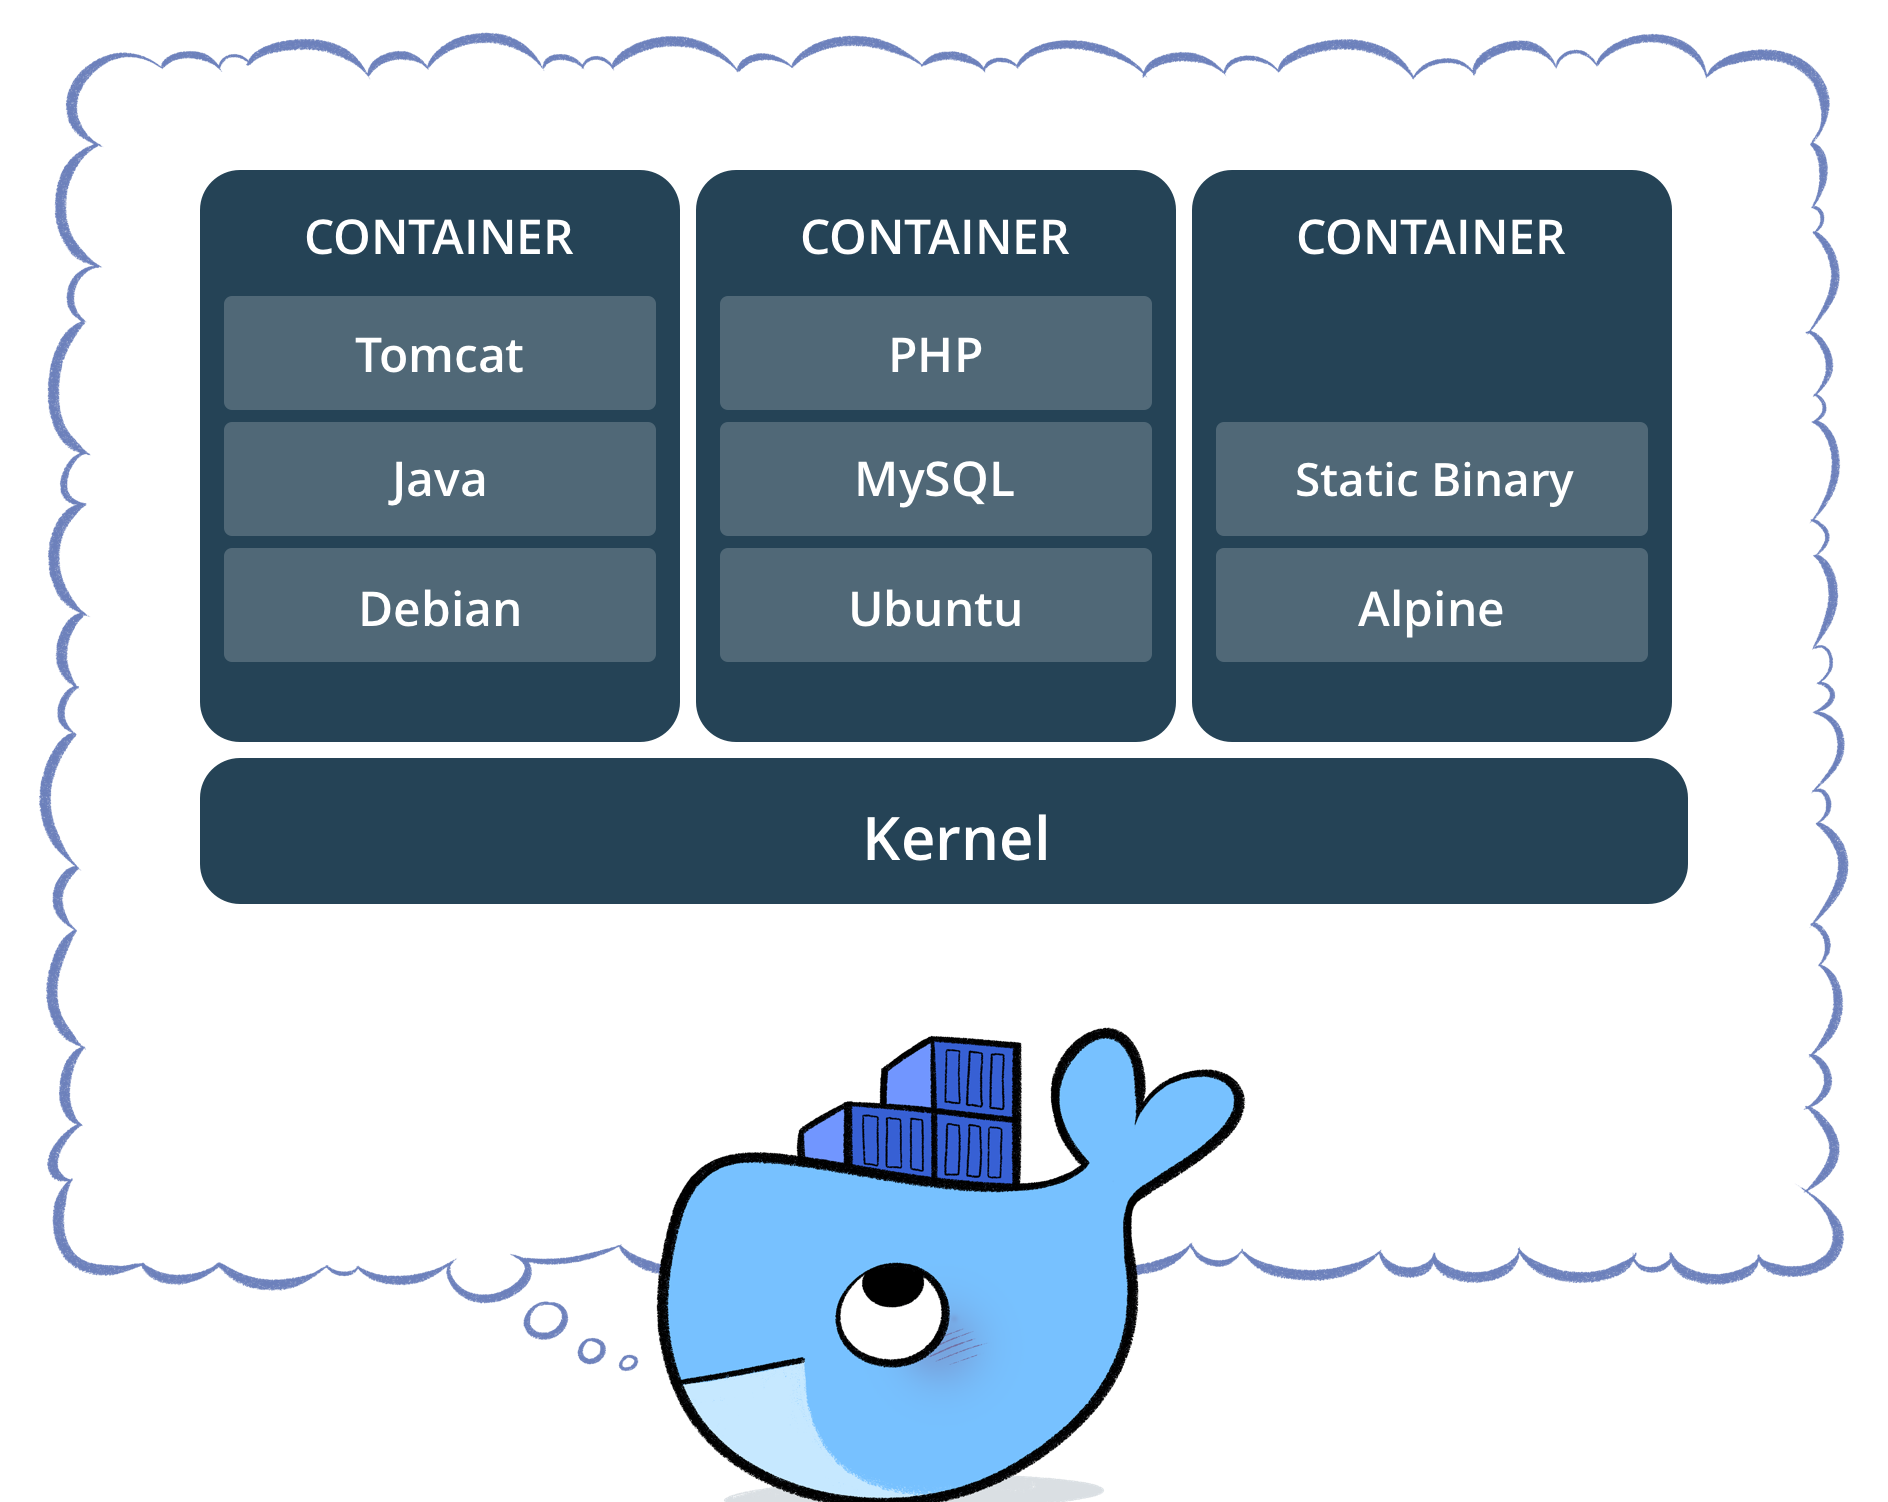
\includegraphics{images/container-1.png}
\caption{Docker Containers}
\end{figure}

Image Source
{[}https://www.docker.com/sites/default/files/Package\%20software\%40x2.png){]}

\subsection{Installing Docker}\label{install-docker}

\subsubsection{Install Docker for OSX}\label{install-docker-for-osx}

In order to install on OSX, you need to do the following steps:

\begin{enumerate}
\def\labelenumi{\arabic{enumi}.}
\item
  Download \texttt{Docker.dmg} file from
  \href{}{https://docs.docker.com/docker-for-mac/install/\#download-docker-for-mac}
\item
  Start \texttt{Docker.app}
\end{enumerate}

\subsubsection{Install Docker Commuinity Edition for
Ubuntu}\label{install-docker-commuinity-edition-for-ubuntu}

In order to instal Docker community edition for Ubuntu, you first have
to setup the repository where it is located. This can be achieved as
follows:

\begin{verbatim}
$ sudo apt-get update

$ sudo apt-get install \
    apt-transport-https \
    ca-certificates \
    curl \
    software-properties-common

$ curl -fsSL https://download.docker.com/linux/ubuntu/gpg | sudo apt-key add -

$ sudo apt-key fingerprint 0EBFCD88

$ sudo add-apt-repository \
   "deb [arch=amd64] https://download.docker.com/linux/ubuntu \
   $(lsb_release -cs) \
   stable"
\end{verbatim}

Now you have configured the repository location, you can install it
after you haved updated the operating system. The update and install is
done as follows:

\begin{verbatim}
$ sudo apt-get update
$ sudo apt-get install docker-ce
$ sudo apt-get update
\end{verbatim}

To check if the Docker works, please follow the following command.

\begin{verbatim}
$ sudo docker run hello-world
\end{verbatim}

\section{Introduction to Kubernetes}\label{introduction-to-kubernetes}

\subsection{Topics Covered and Learning
Outcome}\label{topics-covered-and-learning-outcome-1}

\begin{itemize}

\item
  What is Kubernetes?
\item
  What are containers?
\item
  Cluster components in Kubernetes
\item
  Basic Units in Kubernetes
\item
  Run an example with Minikube
\item
  Interactive online tutorial
\item
  Have a solid understanding of Containers and Kubernetes

  \begin{itemize}
  
  \item
    Understand the CLuster components of Kubernetes
  \item
    Understand the terminology of Kubernetes
  \end{itemize}
\item
  Gain practical experience with kubernetes

  \begin{itemize}
  
  \item
    With minikube
  \item
    With an interactive online tutorial
  \end{itemize}
\end{itemize}

\subsection{What is Kubernetes?}\label{what-is-kubernetes}

Kubernetes is an open-source platform designed to automate deploying,
scaling, and operating application containers.
{[}\href{https://kubernetes.io/docs/concepts/overview/what-is-kubernetes/}{1}{]}

With Kubernetes, you can:

\begin{itemize}

\item
  Deploy your applications quickly and predictably.
\item
  Scale your applications on the fly.
\item
  Roll out new features seamlessly.
\item
  Limit hardware usage to required resources only.
\item
  Run applications in public and private clouds.
\end{itemize}

Kubernetes is

\begin{itemize}

\item
  Portable: public, private, hybrid, multi-cloud
\item
  Extensible: modular, pluggable, hookable, composable
\item
  Self-healing: auto-placement, auto-restart, auto-replication,
  auto-scaling
\end{itemize}

\subsection{What are containers?}\label{what-are-containers}

\begin{figure}
\centering
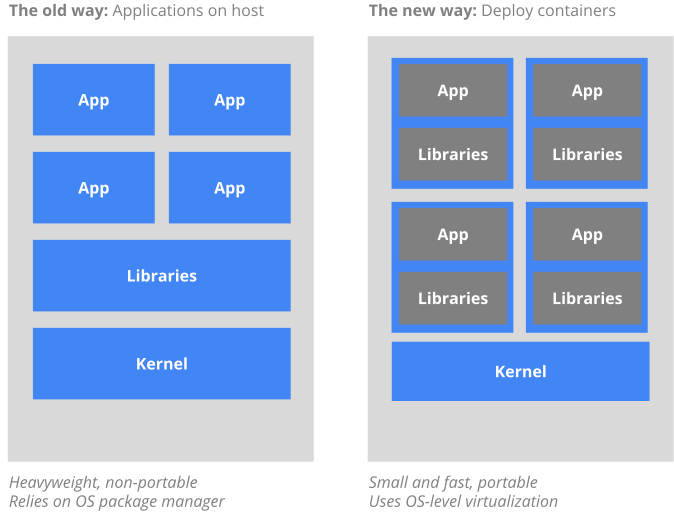
\includegraphics{images/why_containers.svg}
\caption{Kubernetes Containers}
\end{figure}

Image source:
{[}https://d33wubrfki0l68.cloudfront.net/e7b766e0175f30ae37f7e0e349b87cfe2034a1ae/3e391/images/docs/why\_containers.svg{]}

\subsection{Basic Units}\label{basic-units}

\subsubsection{Pods}\label{pods}

A pod (as in a pod of whales or pea pod) is a group of one or more
containers (such as Docker containers), with shared storage/network, and
a specification for how to run the containers. A pod's contents are
always co-located and co-scheduled, and run in a shared context. A pod
models an application-specific ``logical host'' - it contains one or
more application containers which are relatively tightly coupled --- in
a pre-container world, they would have executed on the same physical or
virtual machine.

\subsubsection{Services}\label{services}

Service is an abstraction which defines a logical set of Pods and a
policy by which to access them - sometimes called a micro-service. The
set of Pods targeted by a Service is (usually) determined by a Label
Selector.

\subsubsection{Deployments}\label{deployments}

A Deployment controller provides declarative updates for Pods and
ReplicaSets. You describe a desired state in a Deployment object, and
the Deployment controller changes the actual state to the desired state
at a controlled rate. You can define Deployments to create new
ReplicaSets, or to remove existing Deployments and adopt all their
resources with new Deployments.

\subsection{Run an example with Minikube in
console}\label{run-an-example-with-minikube-in-console}

\begin{enumerate}
\item
  minikube installation
\item
  minikube hello-minikube
\end{enumerate}

\subsubsection{\texorpdfstring{Install
\texttt{minikube}}{Install minikube}}\label{install-minikube}

\paragraph{OSX}\label{osx}

\begin{verbatim}
curl -Lo minikube https://storage.googleapis.com/minikube/releases/v0.25.0/minikube-darwin-amd64 && chmod +x minikube && sudo mv minikube /usr/local/bin/
\end{verbatim}

\paragraph{Linux}\label{linux}

\begin{verbatim}
curl -Lo minikube https://storage.googleapis.com/minikube/releases/v0.25.0/minikube-linux-amd64 && chmod +x minikube && sudo mv minikube /usr/local/bin/
\end{verbatim}

\subsubsection{Start a cluster using
Minikube}\label{start-a-cluster-using-minikube}

\begin{verbatim}
$ minikube start
\end{verbatim}

\subsubsection{Create a deployment}\label{create-a-deployment}

\begin{verbatim}
$ kubectl run hello-minikube --image=k8s.gcr.io/echoserver:1.4 --port=8080
\end{verbatim}

\subsubsection{Expose the service}\label{expose-the-service}

\begin{verbatim}
$ kubectl expose deployment hello-minikube --type=NodePort
\end{verbatim}

\subsubsection{Check running status}\label{check-running-status}

This step is to make sure you have a pod up and running.

\begin{verbatim}
$ kubectl get pod
\end{verbatim}

\subsubsection{Call service api}\label{call-service-api}

\begin{verbatim}
$ curl $(minikube service hello-minikube --url)
\end{verbatim}

\subsubsection{Take a look from
Dashboard}\label{take-a-look-from-dashboard}

\begin{verbatim}
$ minikube dashboard
\end{verbatim}

\subsubsection{Delete the service and
deployment}\label{delete-the-service-and-deployment}

\begin{verbatim}
$ kubectl delete service hello-minikube
$ kubectl delete deployment hello-minikube
\end{verbatim}

\subsubsection{Stop the cluster}\label{stop-the-cluster}

\begin{verbatim}
$ minikube stop
\end{verbatim}

\subsection{Interactive Tutorial
Online}\label{interactive-tutorial-online}

\begin{itemize}
\item
  Start cluster
  https://kubernetes.io/docs/tutorials/kubernetes-basics/cluster-interactive/
\item
  Deploy app
  https://kubernetes.io/docs/tutorials/kubernetes-basics/cluster-interactive
\item
  Explore
  https://kubernetes.io/docs/tutorials/kubernetes-basics/explore-intro/
\item
  Expose
  https://kubernetes.io/docs/tutorials/kubernetes-basics/expose-intro/
\item
  Scale
  https://kubernetes.io/docs/tutorials/kubernetes-basics/scale-intro/
\item
  Update
  https://kubernetes.io/docs/tutorials/kubernetes-basics/update-interactive/
\item
  MiniKube
  https://kubernetes.io/docs/tutorials/stateless-application/hello-minikube/
\end{itemize}
